\chapter{Background and Related Work}
\label{chap:background}

Later chapters build on several technologies and prior systems described here.
Section~\ref{sec:bg-sensor-data} reviews environmental sensor data management and its key challenges.
The OGC SensorThings API standard along with its FROST-Server implementation are covered in
Section~\ref{sec:bg-sta}. Section~\ref{sec:bg-timeio} then analyzes the UFZ Time.IO solution
that served as the starting point for the work. The institutional context behind its selection
is discussed in Section~\ref{sec:bg-elter-context}, and Section~\ref{sec:bg-elter} outlines
the eLTER research infrastructure and its data integration requirements.

%% ================================================================
\section{Environmental Sensor Data Management}
\label{sec:bg-sensor-data}
%% ================================================================

Environmental monitoring deployments typically connect sensors to data loggers or gateways
that forward observations to a central infrastructure. A representative architecture has four layers:
edge devices sampling physical quantities, an ingestion layer receiving data over one or more
protocols, a storage layer optimized for time-series workloads, and an access layer exposing the
data through standardized interfaces \cite{hart2006environmental}.

Heterogeneity across these systems poses a significant engineering challenge. A single monitoring network
may combine sensors from different manufacturers, each using a proprietary payload format, delivered
over MQTT, HTTP~POST, SFTP file upload, or manual CSV import. Temporal resolutions range from
sub-second sampling on vibrating-wire piezometers to daily aggregates from weather stations.
Reconciling these differences into a unified data model is a prerequisite for any cross-site analysis
\cite{horsburgh2008observations}.

Several platforms address parts of this problem space. The Observations Data Model~2 (ODM2)
\cite{horsburgh2016odm2} provides a relational schema for managing diverse observational data with
rich provenance metadata. ERDDAP \cite{simons2023erddap} focuses on data distribution, enabling
scientists to access gridded and tabular datasets through uniform query interfaces. The OGC Sensor
Observation Service (SOS) \cite{ogcsos} defines a standard web-service interface for querying sensor
data, but its XML-based protocol has been largely superseded by the RESTful SensorThings~API discussed
in Section~\ref{sec:bg-sta}.

What these solutions share is the recognition that interoperability standards are essential for
cross-institutional data sharing. Without a shared data model and access protocol, each
integration turns into a bespoke point-to-point effort. The work in this thesis focuses on
the Czech University of Life Sciences Prague (CZU) deployment, where sensors from multiple
manufacturers need to be unified under a single platform accessible to several research groups.

%% ================================================================
\section{OGC SensorThings API}
\label{sec:bg-sta}
%% ================================================================

The OGC SensorThings API (STA) \cite{ogc-sta} is an open standard that defines a RESTful interface
for managing and accessing Internet of Things sensor data. Ratified by the Open Geospatial Consortium in 2016,
it was designed to be lightweight, JSON-based, and suitable for resource-constrained IoT environments ---
in contrast to the earlier XML-heavy Sensor Observation Service.

\subsection{Data Model}
\label{sec:bg-sta-model}

The STA data model is built around six core entity types and their relationships:

\begin{itemize}
  \item \textbf{Thing} --- a physical object of interest, such as a weather station or a water gauge.
        A Thing has a \emph{Location} representing its geospatial position.
  \item \textbf{Datastream} --- a logical grouping of Observations measuring a single
        \emph{ObservedProperty} (e.g.\ water level, air temperature) with a specific \emph{Sensor}.
        Each Datastream belongs to exactly one Thing.
  \item \textbf{Observation} --- an individual measurement event, characterized by a
        \texttt{phenomenonTime} (when the phenomenon occurred), a \texttt{resultTime} (when the
        result was produced), and a \texttt{result} value.
  \item \textbf{Sensor} --- the instrument or procedure that produces Observations.
  \item \textbf{ObservedProperty} --- the physical quantity being measured (e.g.\
        ``Water Temperature'').
  \item \textbf{FeatureOfInterest} --- the real-world feature to which an Observation applies,
        typically derived from the Thing's Location.
\end{itemize}

The standard supports navigation between entities through URL-based association links. For example,
\texttt{/Things(1)/Datastreams} returns all Datastreams belonging to Thing~1, and
\texttt{/Datastreams(5)/Observations?\$filter=phenomenonTime gt 2024-01-01T00:00:00Z}
returns filtered Observations. This query model enables clients to traverse the entity graph
without prior knowledge of the underlying database schema.

STA also defines an MQTT extension (Part~2 of the standard) that allows clients to subscribe to
entity changes in real time, making it suitable for both historical queries and live data streams.

\subsection{STA Server Implementations}
\label{sec:bg-frost}

Several server implementations of the OGC SensorThings API exist. GOST\footnote{GOST SensorThings API server: \url{https://github.com/gost/server}} is a lightweight Go-based implementation focusing on ease of deployment and low resource consumption, but it implements only a subset of the query options and has seen limited maintenance since 2020. SensorThingsServer by 52°North\footnote{52°North SensorThings API: \url{https://github.com/52North/sensorweb-server-sta}} provides STA Part~1 compliance on top of Spring Boot and Hibernate, targeting integration with the broader 52°North sensor web ecosystem, though its community adoption remains smaller. FROST-Server \cite{frost-server}, developed by the Fraunhofer Institute for Optronics, System Technologies and Image Exploitation (IOSB), is the most widely adopted STA implementation and serves as the OGC reference for conformance testing.

FROST-Server was selected for this platform for three reasons. First, the upstream Time.IO system (Section~\ref{sec:bg-timeio}) already integrates FROST-Server, so adopting a different implementation would have required replacing a core component of the inherited stack. Second, FROST-Server provides full STA Part~1 (Sensing) compliance, including \texttt{\$filter}, \texttt{\$expand}, \texttt{\$select}, \texttt{\$orderby}, and \texttt{\$top}/\texttt{\$skip} query options, as well as the MultiDatastream extension for sensors producing multiple observed properties in a single observation. Third, a key architectural property of FROST-Server is that it reads entity data from PostgreSQL views rather than requiring a specific physical table layout. This allows operators to map an existing database schema to the STA entity model by defining appropriate SQL views, a capability that the Time.IO platform exploits through its local STA views, as described in Section~\ref{sec:bg-timeio-arch}.

FROST-Server is deployed as a Java web application on Apache Tomcat\footnote{Apache Tomcat: \url{https://tomcat.apache.org/}} and uses PostgreSQL\footnote{PostgreSQL: \url{https://www.postgresql.org/}} with the PostGIS\footnote{PostGIS spatial extension: \url{https://postgis.net/}} extension as its backing store. Each deployment is configured through a Tomcat context file that specifies the JDBC connection parameters, API version, and plugin settings.

%% ================================================================
\section{The UFZ Time.IO Solution}
\label{sec:bg-timeio}
%% ================================================================

Time.IO (internally referred to as \emph{tsm-orchestration} or TSM) is an open-source environmental
sensor data management platform developed at the Helmholtz Centre for Environmental Research (UFZ)
in Leipzig \cite{bumberger2025timeio,timeio-ref}. It provides an end-to-end pipeline for ingesting, storing,
quality-controlling, and serving environmental time-series data. The platform served as the starting
point for the work described in this thesis.

\subsection{The UFZ TSM Ecosystem}
\label{sec:bg-timeio-ecosystem}

Not a single repository, the UFZ TSM project is a broader ecosystem of over a dozen
components hosted under the \texttt{ufz-tsm} group on the Helmholtz Codebase. The ecosystem comprises three core components, illustrated in Figure~\ref{fig:timeio-ecosystem}: the Sensor Management System (SMS) for metadata registration and management, Time.IO for time-series data ingestion and storage, and the System for automated Quality Control (SaQC) for data analysis and quality assurance. Data enters the system via MQTT or (S-)FTP and is served through the OGC SensorThings API.

\begin{figure}[ht]
  \centering
  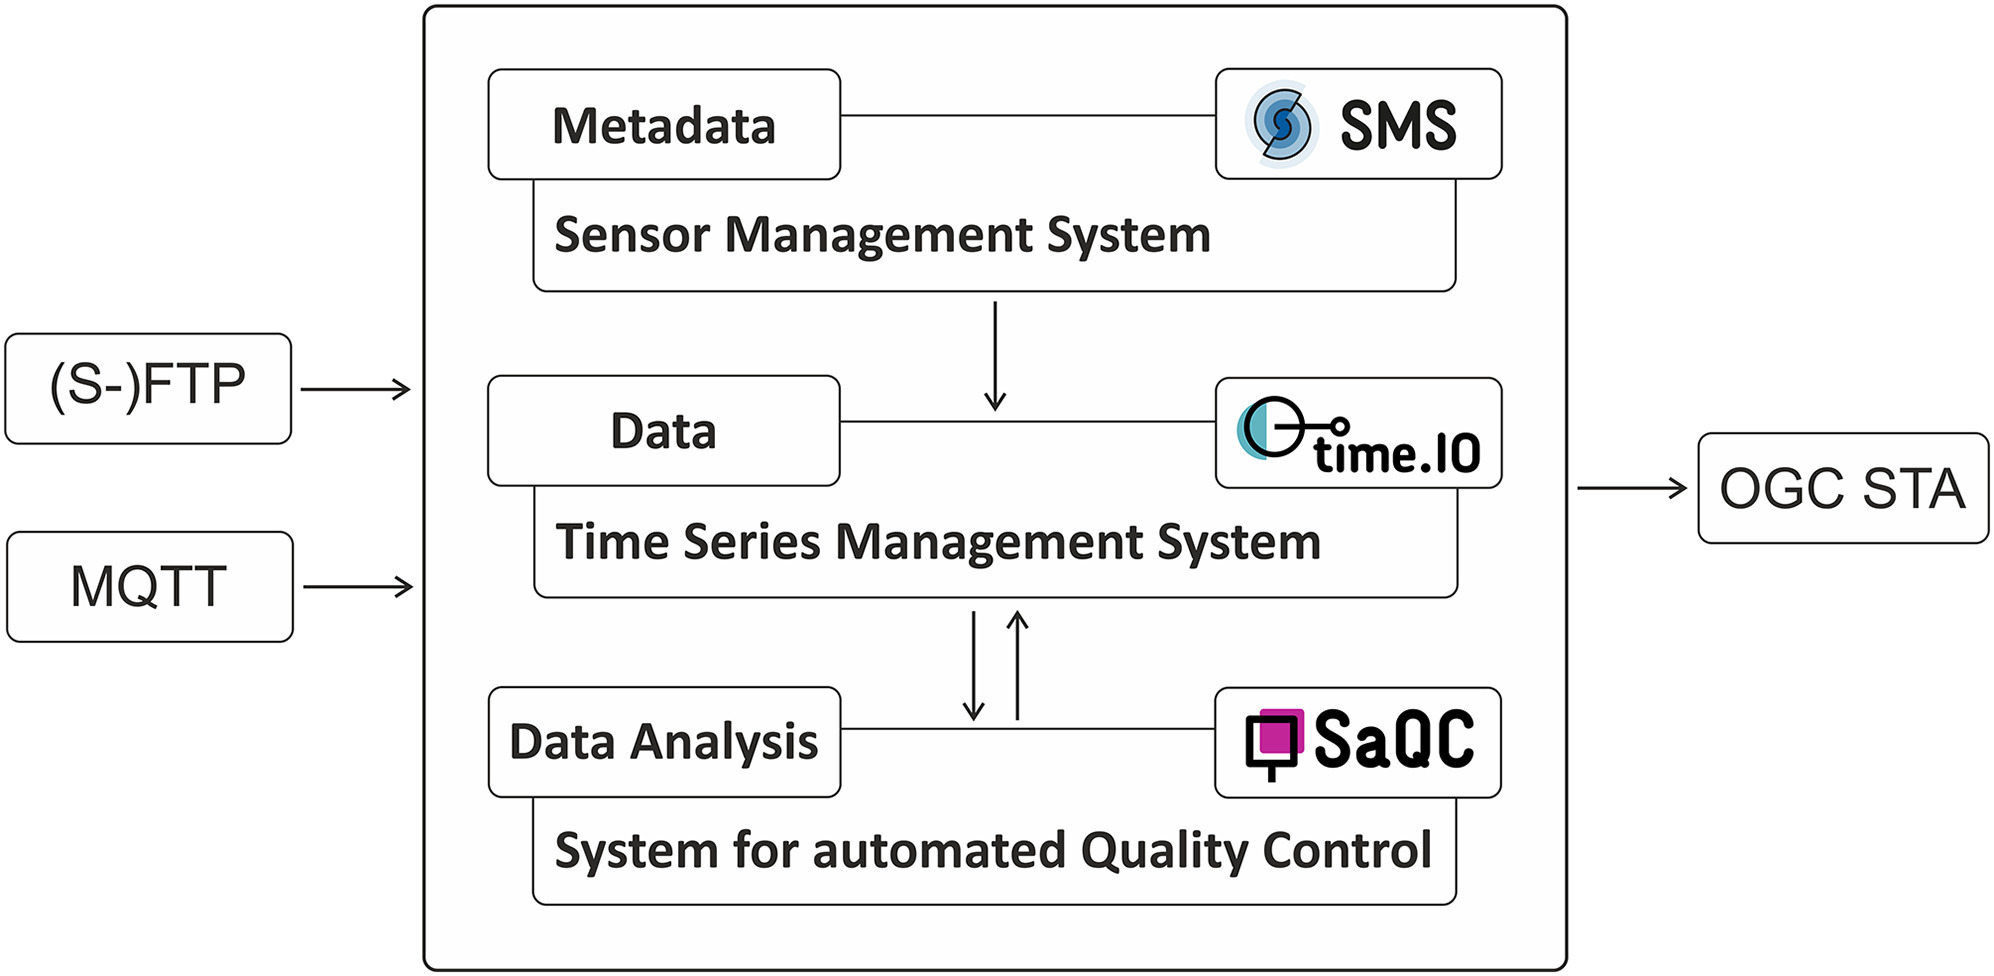
\includegraphics[width=0.85\textwidth]{figures/timeio-ecosystem.jpg}
  \caption{High-level architecture of the UFZ Time.IO ecosystem. \emph{Source: Bumberger et~al.\ \cite{bumberger2025timeio}, reproduced under CC-BY~4.0.}}
  \label{fig:timeio-ecosystem}
\end{figure}

Beyond the
core \texttt{tsm-orchestration} ingestion pipeline adopted in this thesis, the ecosystem
includes two frontend projects (\texttt{tsm-frontend}, a Django\footnote{Django web framework: \url{https://www.djangoproject.com/}} application with 465~commits,
and \texttt{thing-management}, a newer FastAPI/Vue.js\footnote{Vue.js framework: \url{https://vuejs.org/}} replacement started in September~2024),
a combined deployment repository (\texttt{timeio-and-sms}), the external Sensor Management
System (SMS) discussed in Section~\ref{sec:bg-timeio-limitations}, Kubernetes Helm charts,
developer utilities, and several supporting libraries.

This thesis adopts only \texttt{tsm-orchestration} as its foundation. The upstream frontend
components were replaced by the Water Data Platform portal (Chapter~\ref{chap:implementation})
because both upstream frontends produced invalid MQTT configuration messages that broke the
ingestion pipeline, and neither provided the project-oriented management model required by CZU.

\subsection{Architecture Overview}
\label{sec:bg-timeio-arch}

Time.IO is deployed as a set of Docker containers orchestrated by Docker Compose\footnote{Docker Compose: \url{https://docs.docker.com/compose/}}. The infrastructure
layer comprises the following core services:

\begin{itemize}
  \item \textbf{PostgreSQL with TimescaleDB} --- the central database, storing both the configuration
        database (\texttt{config\_db} schema) and per-thing observation data in isolated schemas.
  \item \textbf{Mosquitto\footnote{Eclipse Mosquitto MQTT broker: \url{https://mosquitto.org/}} MQTT broker} --- the event backbone connecting all workers and external
        sensor data sources. Supports both plain (port~1883) and TLS-encrypted (port~8883)
        connections.
  \item \textbf{MinIO object storage} --- an S3-compatible store used for file-based data ingestion.
        Each Thing receives its own bucket for raw data files.
  \item \textbf{FROST-Server} --- an OGC SensorThings API endpoint deployed on Apache Tomcat,
        providing standardized read access to observation data through SQL views over per-thing
        schemas.
  \item \textbf{Keycloak} --- an OpenID Connect identity provider managing user authentication
        and role-based access control.
  \item \textbf{Grafana}\footnote{Grafana visualization platform: \url{https://grafana.com/}} --- a visualization layer with pre-configured dashboards for time-series
        exploration.
  \item \textbf{Flyway}\footnote{Flyway database migration tool: \url{https://flywaydb.org/}} --- a database migration tool that applies versioned SQL scripts to
        initialise and evolve the database schema.
\end{itemize}

On top of these infrastructure services, Time.IO deploys a set of specialized workers and a
configuration API. The workers follow a message-driven architecture: each subscribes to one or more
MQTT topics, performs its designated processing, and optionally publishes results to downstream
topics. This design decouples the components and allows independent scaling and deployment
of each worker.

Its configuration database (\texttt{config\_db} schema) stores the metadata that drives the entire
pipeline. Key tables include \texttt{thing} (sensor device definitions), \texttt{project} (logical
groupings of Things), \texttt{database} (connection credentials per project), \texttt{s3\_store}
(MinIO bucket configuration), \texttt{file\_parser} and \texttt{file\_parser\_type} (parser
definitions), \texttt{mqtt} and \texttt{mqtt\_device\_type} (MQTT ingestion settings), and
\texttt{ext\_api} and \texttt{ext\_sftp} (external data source configurations).

Central to this design is the \emph{per-thing schema} pattern: when a new Thing is provisioned,
the platform creates a dedicated PostgreSQL schema containing its own observation and
datastream tables. The full provisioning sequence and its isolation properties are described
in Section~\ref{sec:arch-db-perthings}.

Upstream FROST-Server integration relies on a set of SQL views
(\texttt{sql/sta\_views/}) that map the STA entity model to tables managed by the external
Sensor Management System (SMS). These views query SMS-provided metadata (device catalogs,
contact records, deployment actions, and datastream links) to construct the
\texttt{THINGS}, \texttt{DATASTREAMS}, \texttt{OBSERVATIONS}, and related entities that
FROST-Server reads. Because the SMS service was never operational
(Section~\ref{sec:bg-timeio-limitations}), these views returned empty result sets or failed
entirely, rendering the STA endpoint non-functional. Without a working STA layer, FROST-Server
could not serve any observation data, effectively breaking one of the platform's core access
interfaces.

\subsection{Worker Architecture}
\label{sec:bg-timeio-workers}

All workers inherit from the \texttt{AbstractHandler} base class defined in the \texttt{timeio.mqtt}
module. This base class manages the MQTT connection lifecycle, health-check heartbeats, and
structured error handling. Each worker subscribes to one or more MQTT topics, performs its
designated processing in the \texttt{on\_message} callback, and optionally publishes results
to downstream topics. This message-driven design decouples the components and allows
independent scaling and deployment.

The platform deploys nine workers covering configuration processing, infrastructure
provisioning, data ingestion (file-based and MQTT-based), quality control, and
synchronization with external data sources. A cron scheduler triggers periodic execution
of the synchronization workers. The full worker catalog with MQTT topics and
responsibilities is presented in Table~\ref{tab:tsm-workers}
(Section~\ref{sec:impl-tsm-workers}).

\subsection{Parser Framework}
\label{sec:bg-timeio-parsers}

The data parsing subsystem uses a pluggable architecture based on an abstract base class
(\texttt{AbcParser}) with concrete implementations registered in a parser map. The framework
distinguishes between file parsers (used by the file-ingest worker for uploaded CSV and JSON
files) and MQTT parsers (used by the mqtt-ingest worker for real-time device payloads).

File parsers include a general-purpose CSV parser (\texttt{CsvParser}), a JSON parser
(\texttt{JsonParser}), and a Pandas-based parser (\texttt{PandasParser}) for complex
tabular transformations. MQTT device parsers are specialized for specific hardware:
\texttt{ChirpStackGenericParser} handles LoRaWAN payloads from the ChirpStack\footnote{ChirpStack LoRaWAN network server: \url{https://www.chirpstack.io/}} network server,
\texttt{CampbellCr6Parser} processes GeoJSON-formatted data from Campbell Scientific CR6 loggers,
\texttt{YdocMl417Parser} handles Ydoc ML-417 water quality sensors, and
\texttt{BrightskyDwdApiParser} parses German Weather Service API responses. A
\texttt{SineDummyParser} generates synthetic sine-wave data for testing.

Each parser produces a list of \texttt{Observation} objects with fields for timestamp, value, origin,
position (identifying the Datastream), and column header. Observations support four result types:
boolean, number, string, and JSON.

Critically, all parsers and device types in the upstream platform are hardcoded in the Python
source code. Adding support for a new sensor model or file format requires implementing a new
parser class, registering it in the parser map, rebuilding the Docker image, and redeploying
the affected worker. There is no mechanism for operators or end users to define new parsers,
MQTT device types, or file-parsing configurations at runtime through a management interface.
The database schema also lacks extensibility: the \texttt{mqtt\_device\_type} and
\texttt{ext\_api\_type} tables have no metadata columns, so any device-specific configuration
must be baked into the parser source code. This rigidity is a significant limitation for
deployments that must accommodate diverse and evolving sensor hardware.

\subsection{Current State and Limitations}
\label{sec:bg-timeio-limitations}

At the time this work commenced, Time.IO exhibited several limitations that directly
motivated the contributions of this thesis. These limitations span the SMS integration, the
upstream frontend solutions, and the overall project maturity.

\paragraph{Sensor Management System.}
The most significant limitation concerned the Sensor Management System (SMS), an external metadata
service intended to provide controlled vocabularies, semantic annotations, and a catalog of sensor
descriptions. The SMS was designed to be the authoritative source of Thing metadata for FROST-Server,
with dedicated SQL views (\texttt{sql/sta\_views/}) mapping SMS-managed entities to the STA data model.
However, the SMS service was never operational. The synchronization worker
(\texttt{sync\_sms\_manager.py}) existed in the codebase, but the upstream SMS backend it depended on
was not available. Without populated SMS tables, the STA views returned empty result sets or failed
to execute, rendering FROST-Server unable to serve any observation data. This was not a minor feature
gap: the STA endpoint is a core access interface of the platform, and its absence made the upstream
TSM deployment effectively non-functional for any client expecting standards-compliant data access.

The \texttt{timeio-and-sms} combined deployment repository, which was intended to demonstrate
the integrated SMS and Time.IO workflow, proved impossible to deploy successfully. Multiple
dependencies were outdated or no longer available, and the solution contained breaking bugs that
prevented the services from starting. The repository's documentation was partially written in
German and reflected an internal prototype rather than a production-ready integration. With only
175~commits total and activity ceasing in July~2024, the combined SMS deployment did not represent
a viable path forward.

\paragraph{Upstream frontends.}
The original \texttt{tsm-frontend} (Django) provided basic Thing management functionality but
contained bugs that caused inconsistencies between the frontend configuration forms and the
ingestion pipeline's expectations. When a Thing was created or modified through the Django
interface, the resulting MQTT configuration messages did not always match the format and content
that the downstream workers (\texttt{configdb-updater}, \texttt{thing-setup}) expected, leading
to silent failures in infrastructure provisioning.

The newer \texttt{thing-management} replacement (Vue.js~3 + FastAPI) was still in early development
at the time of this work, with limited functionality and similar integration issues. The
frontend's MQTT message generation contained bugs that caused several core ingestion workflows
, particularly file-based ingestion and external API synchronization, to fail. Neither
upstream frontend provided project-based multi-tenancy, role-based access control beyond basic
Helmholtz~AAI group membership, alerting, geospatial layer management, or internationalization
--- all of which were required for the CZU deployment.

\paragraph{Upstream project activity.}
Beyond the specific component issues, the upstream TSM ecosystem showed an overall pattern of
fragmented development. The codebase was distributed across more than a dozen repositories with
varying levels of maturity. The FETA module (\texttt{timeio/feta.py}), which provides an ORM-like
abstraction over the configuration database, was actively maintained and central to the worker
architecture. However, higher-level management features were either absent, buggy, or spread
across multiple partially overlapping projects (\texttt{tsm-frontend} vs.\ \texttt{thing-management}).

The platform lacks several capabilities required for the CZU deployment: project-based
multi-tenancy with role-based access, an alert and notification system, geospatial layer management,
a user-facing portal for sensor configuration and data exploration, and batch CSV import with
configurable parsing. These gaps are analyzed in Chapter~\ref{chap:requirements} and addressed
by the contributions described in Chapters~\ref{chap:architecture} and~\ref{chap:implementation}.

%% ================================================================
\section{Institutional Context: eLTER and the Adoption of Time.IO}
\label{sec:bg-elter-context}
%% ================================================================

The eLTER network relies on a shared digital layer called the eLTER CyberInfrastructure
(eLTER~CI), described in Section~\ref{sec:bg-elter-ci}. The UFZ is a core contributor to
this infrastructure: it develops and operates Time.IO as the time-series data acquisition
component of the eLTER~CI, handling ingestion, storage, quality control, and STA-based
access for environmental observations. The work is carried out under the EU Horizon~2020
eLTER~PLUS project (Grant Agreement No.~871128, 2020--2025), which funds the build-up of
the eLTER~CI and its validation through pilot deployments at real monitoring sites across
Europe.

The Czech University of Life Sciences Prague (CZU) operates hydrological and meteorological
monitoring networks across several catchment areas in the Czech Republic and aspires to
join the eLTER network as a recognized site. Its data management requirements ---
consolidating heterogeneous sensors under a single standards-compliant platform with
project-based multi-tenancy --- overlap closely with what Time.IO was built to provide.
Within the eLTER~PLUS project, CZU's deployment was established as a pilot: a test of
whether Time.IO can serve operational needs beyond UFZ's own sites and whether the
resulting extensions can feed back into the shared eLTER~CI.

This pilot arrangement defines the scope of the thesis. The work builds on a fork of
\texttt{tsm-orchestration} rather than a new platform, and the extensions described in
later chapters are designed with upstream contribution in mind. Building on Time.IO ties
the CZU deployment into the broader eLTER adoption path, but it also means inheriting
the limitations documented in Section~\ref{sec:bg-timeio-limitations}.

%% ================================================================
\section{eLTER Research Infrastructure}
\label{sec:bg-elter}
%% ================================================================

The European Long-Term Ecosystem, Critical Zone and Socio-Ecological Research Infrastructure
(eLTER~RI) \cite{elter-ref} coordinates environmental monitoring across more than 400~sites
in over 25~European countries. Sites range from alpine observatories and forest flux towers
to freshwater catchments and urban gradient transects. The network distinguishes two
categories: \emph{eLTER Sites}, which carry out long-term observations at the ecosystem
level, and \emph{eLTER Platforms}, which host intensive, high-resolution measurement campaigns
on shorter time scales. eLTER is currently transitioning from project-funded development
under eLTER~PLUS toward sustained operation as a European Research Infrastructure
Consortium (ERIC).

\subsection{eLTER CyberInfrastructure}
\label{sec:bg-elter-ci}

Connecting these distributed sites into a coherent research environment is the
role of the eLTER CyberInfrastructure (eLTER~CI), developed under the eLTER~PLUS
project. The eLTER~CI is designed as an integrated service environment --- not a
loose federation of tools --- where data, metadata, and user-facing applications
share a common identity layer, aligned metadata structures, and coordinated
workflows spanning dataset submission through quality control, curation, discovery,
and analytical use.

The CI supports two complementary data pathways. On the \emph{provider side},
site operators submit datasets (or have them harvested from external repositories),
complete metadata according to an eLTER-specific profile, pass automated quality
checks, and publish records through a curator-mediated review. On the
\emph{consumer side}, researchers discover datasets by site or observed property,
inspect them against controlled vocabularies, access the data through
standardized service endpoints, and perform analysis in managed compute
environments. The main components that implement these pathways are:

\begin{itemize}
  \item \textbf{eLTER~LogIn} --- a federated identity and access service built on
        Perun~AAI, supporting institutional login via eduGAIN, EGI~Check-in, ORCID,
        and Google. A single consolidated identity per user spans all CI services,
        with role-based access control distinguishing data providers, curators,
        researchers, and administrators.
  \item \textbf{Digital Asset Register (DAR)} --- the central dataset repository,
        built on InvenioRDM. It handles registration, metadata curation (using an
        eLTER-specific metadata model), automated quality checks orchestrated by
        Argo~Workflows, and publication with DOI minting through DataCite. A
        harvesting subsystem retrieves metadata from external repositories
        (B2SHARE, Zenodo, and others) so that externally stewarded datasets
        also appear in the eLTER catalog.
  \item \textbf{DEIMS-SDR} --- the Site and Dataset Registry at
        \texttt{deims.org}, serving as the authoritative source of site-level
        metadata: geographic boundaries, instrumentation, observed properties,
        and responsible organizations. Dataset records in the DAR link to
        DEIMS-SDR site identifiers.
  \item \textbf{Vocabulary services} --- controlled terminologies (EnvThes for
        observed properties, eLTER Standard Observations, eLTER Controlled Lists)
        published through SKOSMOS and Apache Jena. These enable consistent
        semantic annotation across sites and disciplines.
  \item \textbf{Online data services} --- Time.IO (TimescaleDB-based) for
        time-series access and Spatial.IO (GeoServer-based) for geospatial
        layers, both linked to DAR records through an Online Asset Register (OAR)
        so that dataset metadata and data access remain connected.
  \item \textbf{DataLabs} --- a JupyterHub-based analytical environment running
        on the CI compute cluster, offering pre-built images (Python, R/RStudio,
        TensorFlow with optional GPU access) for dataset preprocessing,
        transformation, and exploratory analysis.
\end{itemize}

The entire stack runs on Kubernetes and is operated through a GitOps workflow,
making deployments reproducible and auditable. This architecture is directly
relevant to the present work: the CZU deployment is intended to function as a
site-level data acquisition node within the eLTER~CI, with observations
ingested through Time.IO ultimately discoverable and accessible through the DAR
and the associated online services.

\subsection{Implications for Site-Level Deployments}
\label{sec:bg-elter-implications}

Several properties of the eLTER~CI directly constrain what a site-level platform must provide.
Data served to the network must be accessible through the OGC SensorThings API, which the
eLTER~CI has adopted as its candidate standard for real-time sensor data. Sites must
describe their sensors and observed properties using eLTER's controlled vocabularies so that
cross-site queries return semantically comparable results. Authentication must support federated
identity providers compatible with the eLTER~LogIn service. At the same time, individual sites
retain operational independence --- they choose their own sensor hardware, data collection
procedures, and local infrastructure --- so the platform must accommodate heterogeneous
configurations rather than mandating a specific vendor or format.

The gaps between the current CZU deployment and a production-ready eLTER integration ---
including vocabulary alignment, cross-site federation, and FAIR metadata compliance ---
are assessed in Section~\ref{sec:test-deployment-elter}.
